%% This is a skeleton file demonstrating the use of IEEEtran.cls (requires IEEEtran.cls version 1.8a or later) with an IEEE conference paper.
%%
%% Modified by Khan Reaz( kahn.reaz@ieee.org)
%% Support sites:
%% http://www.ieee.org/

%%***********************************************************
%% Legal Notice:
%% This code is offered as-is without any warranty either expressed or implied; without even the implied warranty of MERCHANTABILITY or FITNESS FOR A PARTICULAR PURPOSE! 
%% User assumes all risk and can modify as s/he wants.

%%***********************************************************

%package list
\documentclass[conference]{llncs}
\usepackage{cite}
\usepackage{graphicx}
\graphicspath{ {images/} }

\usepackage{algorithm}
\usepackage{algpseudocode}
\usepackage{mdwmath}
\usepackage{amsmath}
\usepackage{mdwtab}
\usepackage[utf8]{inputenc}
\usepackage[english]{babel}



\begin{document}

%Here goes the title

\title{Analysing Distributed Ledger Mechanisms}


%Authors List

% \author
% {\IEEEauthorblockN{Sourav Das}
% \IEEEauthorblockA{National University of Singapore\\
% souravdas1547@gmail.com}
% }
\maketitle


\begin{abstract}
Abstract goes here
\end{abstract}


\section{Objective}
\label{sec:objective}
We want to write a paper that systematically studies the existing research on Blockchain space and put forwards future research directions. The methodology and approaches adopted in this work can be considered  complementary to existing work  \cite{bano2017consensus}, \cite{joshi2018survey}. The methodologies adopted in this study will be as follows.

First, we identify, devise and systematize the fundamental component that every {\em Distributed Ledger Mechanism} (DLM) attempts to achieve. We present DLM in the fundamental setting by leaving the details involved from a application point of view. Through this modelling we identify the fundamental component and bear minimum assumptions required to solve the problem of DLM. This includes

\begin{itemize}
    \item Underlying Network considerations like synchrony assumptions from best with immediate synchronous to a fully asynchronous assumptions
    \item A total ordering scheme aka consensus mechanism ranging from assuming existence of a global random string
    \item We also considers the spectrum based on finality of the ledger which ranges from BFT based where data are final immediately and PoW based system which the finality is theoretically never achieved.
    \item Information about peers in the system which includes 1) Number of nodes 2) Whether PKI is available or not 3) Dynamic topology
    \item Nature of participants more specifically considering internal attacker or external attacker. In case of non-byzantine nodes are these nodes rational or honest i.e do any system model these system in a BAR setting.
    \item Incentive mechanisms which are strong enough to tolerate across multiple rounds in the protocol
\end{itemize}

We then present qualitative analysis sometime with provable results that how under suitable assumptions of the above properties difficulty of a system design varies. This includes showing that under very strong assumptions the problem meeting the requirements can be met trivially and when are provably impossible. We further identify suitable places for existing work in this spectrum and identify situations about which the community only speaks in a evasive manner or does talk about all. 

Additionally we compare and contrast DLM with Traditional Byzantine Agreement \cite{lamport1982byzantine} where we identify subtle differences that are often overlooked. We also identify the approximations made in DLM research to bypass the impossibilities considered in traditional consensus research. We then discuss difficulties associated with adopting well developed techniques from legacy distributed systems in blockchain research. Lastly we collect several evidences of attempt to ``re-invent the wheel" or attempt of solve open problems in the blockchain community that are already well studied in legacy distributed system. 



% First, we present a abstract model of contemporary  blockchain based system and show that (almost) all can be modelled on a basic underlying structure. We identify the components of this structure, categories them hierarchically and analyze them. 

% First we define what a public ledger system is, who are the participants and what are the requirements of the system. Given this our study shows that at the core, blockchain system can be thought of consisting a bunch of simplified modelling of a distributed public ledger 

Second, we observed that security guarantees of major contemporary blockchain only consider the the {\em static} nature of the system. 
By static here we refer to the property of the blockchain only for a single round, where round could be generation of a single block by PoW, PoS or PBFT as in \cite{gervais2016security}. 
With detailed scenarios, we then discuss why it is equally important to analyze security guarantees of dynamic nature of a blockchain. These includes identifying situations like (1) Rich getting richer, (2) A byzantine adversary adopting extreme strategies to create imbalances in the system.  

% Second, Dynamic nature of blockchains
% We then formally analyze blockchain as a dynamic system spanning across multiple rounds or blocks which is usually left out in majority of the existing work and design. In this we define notion of stability of the system in a dynamic nature \begin{itemize}
%     \item Do rich get richer in this system?
% \end{itemize} 

Third, Security guarantees of a majority of the existing blockchain today rely on considerably unrealistic assumptions about nature of the participants in the system. 
Specifically, these assumption about nature of the participants falls in two categories First, a combination of Byzantine and honest which is considered by majority of existing work and Second, all participants are rational i.e trying to maximize their utility at all times. 
Through a number of different constructive arguments, we show that why alturistic assumptions about a large fraction up to $\frac{3}{4}$ of the participants are unpragmatic. 
Additionally, considering all participants to be rational possibly make the system vulnerable to a very small fraction ,$\frac{1}{10}$th of byzantine participants are sufficient to cause fatal attacks in the system.
Considering above, we make conjecture regarding consideration of a {\em Byzantine Alturistic and Rational} (BAR) participant model provide better security. We end discussion on this topic by identifying interesting open research challenges that one will incur if they consider the BAR adversarial model. 


Fourth, A recent line of work considered a interesting attacks on the overlay networks on blockchain \cite{apostolaki2017hijacking, heilman2015eclipse} which reflects the importance of considering network layer security in blockchain system. One important attack to consider is Denial-of-Service (DoS) on participants of a blockchain. We identify situations in major PoS based blockchains like Algorand \cite{gilad2017algorand} where unless some security practice are followed by users, they become more prone to DoS attacks which eventually lead attacks on the entire system. 

Fifth, We also survey the research progress in interoperability among multiple blockchains starting with atomic swaps to arbitrary data transfer. Here we point out a set of existing problems in blockchain research that can be solved if an efficient mechanism for blockchain interoperablity is solved. We also highlight a vast potential future applications which can be built on top of this system. Our study shows, that only a handful of attempts had been made take this area further leaving out a large number of research problem to address. We finally conclude the discussion on this topic by listing out major challenges in building efficient scalable interoperable system.


Sixth, we proceed to analyze blockchain throughput scalability approaches which adopts the methodologies of sharding and replacing chain by Directed Acyclic Graphs (DAG). 
In doing so, we compare them with scaling throughput by increasing block size, reducing inter-arrival time between each blocks or both. Interestingly, we realize that unless the problem of state-sharding is solved, the above mentioned approaches close reminiscent to increasing throughput by increasing blocksize. We proceed to survey the state of state sharding and analyze the difficulties associated with these approach. Recall, that traditional Peer-to-Peer (P2P) distributed system already address this issue developing seminal tools like Chord \cite{stoica2001chord}, Kademila \cite{ maymounkov2002kademlia}, Pastry \cite{rowstron2001pastry} etc. Hence one might falsely think of state-sharding is a already solved problem. Thus we highlight out the differences between the legacy P2P distributed systems to DLM to identify various open research problem to address.  

Lastly, another interesting recent line of research to solve the limitation of the amount of computation a smart contract can process. Luu et al. introduced the concept of 
Verifier's Dilemma \cite{luu2015demystifying} which shows that this limitation can't be arbitrarily increased without making fundamental design changes. 
A recent line of work \cite{teutsch2017scalable, kalodner2018arbitrum, yoda} starting with Truebit \cite{teutsch2017scalable} attempts to address this problem delegating execution of smart contract with large computation off-chain. 
Arbitrum \cite{kalodner2018arbitrum} formalizes the model presented by Truebit improving upon incentive structure of the mechanism designed as works in the threat model of all rational node as in Truebit. 
YODA \cite{yoda} takes a steps further to solve the problem in a BAR threat model tolerating upto $\frac{1}{2}$ Byzantine adversary. 
This approach still requires multiple parties to execute these contracts which is still far away from ideal model of smart contract execution system analogous to off-chain payment channels \cite{poon2016bitcoin} . We will specify in more detail about the above mentioned approach and open research challenges in further sections.


% In this work, we don't consider research on privacy preserving blockchains that considers anonymity of users, secrecy of smart contract execution and corresponding data. Privacy preserving blockchain is a very important research challenge to solve and we will consider a survey on it as a future work. 






% Third, we try to co-relate existing Proof-of-work and Proof-of-Stake and show that this two schemes are replaceable with each other for all known benefits and attacks. Here we provide mechanisms which shows that for all in the presence of a suitable oracle we show that all existing properties or PoS can be simulated using PoW and visa vis. 




\section{Incentive Compatibility}
The security concerns arising due to Rationality of miners has been considered in the following paper. Theh Highlight
\begin{itemize}
    \item Hostile Bitcoin Takeover \cite{bonneau2018hostile}
    \item Instability withou block reward \cite{carlsten2016instability}
    \item Double spending via whale transactions \cite{liao2017incentivizing}
    \item Selfish mining attack \cite{eyal2016bitcoin}
    \item Why buy when you can rent \cite{bonneau2016buy}
\end{itemize}

The above suggests the need for mechanisms designs which are incentive compatible. We further conjecture that building decentralized permissionless system requires incentive compatibility built in it. Major works have considered the extremes where they only consider a mixture of 
\section{Related Work}
\label{sub:related}
A temporal blockchain: a formal analysis \cite{dennis2016temporal}

A Survey on Consensus Mechanisms and Mining Management in Blockchain Networks \cite{wang2018survey}

Consensus in the age of blockchains \cite{bano2017consensus}

A survey on the security of blockchain systems \cite{li2017survey}


A survey on security and privacy issues of blockchain technology \cite{joshi2018survey}

% \subsection{Internet of Thing setting}
% Blockchain in internet of things: challenges and solutions \cite{dorri2016blockchain}

% Blockchain for IoT security and privacy: The case study of a smart home \cite{dorri2017blockchain}




   

    

%example for inserting image
% \begin{figure}[h]
%   \centering
%   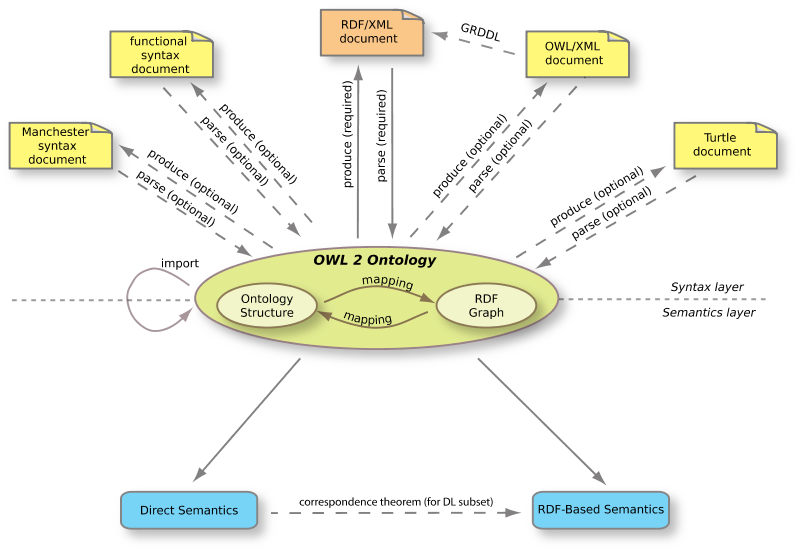
\includegraphics[scale=.45]{OWL2}
%     \caption{The structure of OWL2}
%     \label{fig:OWL2}
% \end{figure}




\bibliographystyle{splncs04}
\bibliography{references}

\end{document}